% ============================================================
% HSBI Beamer — ISLP Lecture Series — IMPROVED EDITION
% Chapter 6: Linear Model Selection and Regularisation
% ============================================================
\documentclass[aspectratio=169,11pt]{beamer}
\usepackage[utf8]{inputenc}\usepackage[T1]{fontenc}\usepackage[english]{babel}
\usepackage{graphicx}\usepackage{booktabs}\usepackage{amsmath,amssymb,amsfonts}
\usepackage{mathtools}\usepackage{hyperref}\usepackage{xcolor}
\usepackage{verbatim}\usepackage{alltt}
\usepackage{tikz}\usetikzlibrary{calc,arrows.meta,positioning,shapes}
\usepackage{tcolorbox}\tcbuselibrary{skins}

\usetheme{Madrid}\usecolortheme{default}
\setbeamertemplate{navigation symbols}{}
\setbeamertemplate{footline}[frame number]
\setbeamertemplate{blocks}[rounded][shadow=false]
\setbeamertemplate{headline}{%
  \leavevmode\hbox{%
    \begin{beamercolorbox}[wd=\paperwidth,ht=2.2ex,dp=0.9ex]{section in head/foot}%
      {\fontsize{4.6}{5.2}\selectfont%
       \insertsectionnavigationhorizontal{\paperwidth}{}{\hskip0pt plus1filll}}%
    \end{beamercolorbox}}%
}
\setbeamerfont{section in head/foot}{size=\tiny}
\setbeamerfont{palette primary}{size=\tiny}
\setbeamerfont{palette tertiary}{size=\tiny}
\setbeamerfont{section in toc}{size=\footnotesize}

\usepackage{listings}
\definecolor{pyKw}{RGB}{0,0,180}\definecolor{pyStr}{RGB}{20,120,40}
\definecolor{pyCom}{RGB}{120,120,120}\definecolor{accent}{RGB}{38,70,140}
\lstdefinestyle{Pystyle}{language=Python,basicstyle=\ttfamily\footnotesize,
  keywordstyle=\color{pyKw}\bfseries,commentstyle=\color{pyCom}\itshape,
  stringstyle=\color{pyStr},showstringspaces=false,upquote=true,
  columns=fullflexible,breaklines=true,literate={~}{{$\sim$}}1}
\lstset{style=Pystyle}

\usepackage{etoolbox}
\makeatletter
\patchcmd{\beamer@sectionintoc}{\vskip1.5em}{\vskip.6em}{\typeout{TOCPATCH-OK}}{\typeout{TOCPATCH-FAIL}}
\makeatother

\AtBeginSection[]{\begin{frame}{Outline}\footnotesize
  \tableofcontents[currentsection,sectionstyle=show/shaded,subsectionstyle=show/show/hide]
\end{frame}}

\newcommand{\islpsource}[1]{%
  \vfill\hfill{\tiny\itshape\color{gray}Source: #1 \textemdash{} ISLP, James et al.\ (2023).}\par
}

\newtcolorbox{takeaway}[1][Takeaway]{enhanced,colback=green!4,colframe=green!50!black,
  boxrule=0pt,leftrule=2.5pt,arc=2pt,fonttitle=\bfseries,title=#1,
  left=2mm,right=2mm,top=1mm,bottom=1mm}
\newtcolorbox{numexample}[1][Worked example]{enhanced,colback=orange!4,colframe=orange!70!black,
  boxrule=0pt,leftrule=2.5pt,arc=2pt,fonttitle=\bfseries,title=#1,
  left=2mm,right=2mm,top=1mm,bottom=1mm}
\newtcolorbox{readme}[1][How to read this]{enhanced,colback=blue!4,colframe=accent,
  boxrule=0pt,leftrule=2.5pt,arc=2pt,fonttitle=\bfseries,title=#1,
  left=2mm,right=2mm,top=1mm,bottom=1mm}

\title{An Introduction to Statistical Learning}
\subtitle{Chapter 6: Linear Model Selection and Regularisation \textemdash{} Improved Edition}
\author{Prof.\ Dr.\ Christoph Weisser}\institute{HSBI}
\date{Summer Semester 2026}\graphicspath{{images/}}

\newtcolorbox{exercise}[1][Exercise]{enhanced, fontupper=\footnotesize, colback=purple!4, colframe=purple!55!black, boxrule=0pt, leftrule=2.5pt, arc=2pt, fonttitle=\bfseries, title=#1, left=2mm, right=2mm, top=1mm, bottom=1mm}
\newtcolorbox{solutionbox}[1][Solution]{enhanced, fontupper=\footnotesize, colback=teal!5, colframe=teal!55!black, boxrule=0pt, leftrule=2.5pt, arc=2pt, fonttitle=\bfseries, title=#1, left=2mm, right=2mm, top=1mm, bottom=1mm}
\newtcolorbox{longexercise}[1][Extended exercise (15 min)]{enhanced, fontupper=\footnotesize, colback=violet!6, colframe=violet!55!black, boxrule=0pt, leftrule=3pt, arc=2pt, fonttitle=\bfseries, title=#1, left=2mm, right=2mm, top=1mm, bottom=1mm}

% Reclaim ~2pt of body height (custom nav headline makes full slides tip over by ~1.83pt)
\addtobeamertemplate{frametitle}{}{\vspace{-2pt}}

\newtcolorbox{labnote}[1][Run this live in the lab notebook]{enhanced, fontupper=\footnotesize, colback=cyan!7, colframe=cyan!45!black, boxrule=0pt, leftrule=3pt, arc=2pt, fonttitle=\bfseries, title=#1, left=2mm, right=2mm, top=1mm, bottom=1mm}

\begin{document}
\begin{frame}[plain]\titlepage\end{frame}

\begin{frame}{The course at a glance}
  \footnotesize
  \begin{center}
  \begin{tabular}{@{}c r l@{}}
    & \textbf{Lecture} & \textbf{Topic}\\
    \midrule
     & 1 & Ch.\ 1 + 2 --- Introduction; what is statistical learning \\
     & 2 & Ch.\ 2 --- Accuracy, bias--variance, Bayes classifier, KNN \\
     & 3--4 & Ch.\ 3 --- Linear regression (estimation, inference, diagnostics) \\
     & 5--6 & Ch.\ 4 --- Classification (logistic, LDA/QDA, naive Bayes, ROC) \\
     & 7 & Ch.\ 5 --- Resampling (validation, CV, bootstrap) \\
    $\blacktriangleright$ & \textbf{8} & \textbf{Ch.\ 6 --- Model selection and regularisation (ridge, lasso)} \\
     & 9 & Ch.\ 7 --- Moving beyond linearity (splines, GAMs) \\
     & 10 & Ch.\ 8 --- Tree-based methods (trees, forests, boosting) \\
     & 11 & Ch.\ 10 --- Deep learning (MLPs, CNNs, training) \\
     & 12 & Ch.\ 13 --- Multiple testing (FWER, FDR) \\
  \end{tabular}
  \end{center}
  \vspace{2pt}
  {\scriptsize Twelve sessions of 180 minutes. $\blacktriangleright$ marks today's chapter. Short exercises every $\sim$20 min; extended exercises every $\sim$45 min; each chapter has a companion lab notebook.}
\end{frame}


\begin{frame}{Contents}\small
  \tableofcontents[hideallsubsections]
\end{frame}

\begin{frame}{Notation in this chapter}
  \footnotesize
  \begin{center}
  \begin{tabular}{@{}ll@{}}
    \toprule
    \textbf{Symbol} & \textbf{Meaning} \\
    \midrule
    $d$ & Number of predictors in a candidate model ($2^p$ subsets in total) \\
    $\mathrm{RSS}$, $\mathrm{TSS}$ & Residual / total sum of squares \\
    $\hat\sigma^2$ & Estimated noise variance \\
    $C_p$, AIC & $\tfrac1n(\mathrm{RSS} + 2d\hat\sigma^2)$ --- lighter complexity penalty \\
    BIC & $\tfrac1n(\mathrm{RSS} + \log(n)\,d\hat\sigma^2)$ --- heavier penalty \\
    adj.\ $R^2$ & $R^2$ corrected for the model size $d$ \\
    $\lambda$ & Tuning parameter: penalty strength, chosen by CV \\
    $\lambda\sum_j \beta_j^2$ & Ridge ($\ell_2$) penalty: shrinks, never exactly zero \\
    $\lambda\sum_j |\beta_j|$ & Lasso ($\ell_1$) penalty: shrinks and selects \\
    $Z_m$, $\phi_{jm}$ & Derived components and their loadings \\
    $M$ & Number of components used in PCR / PLS \\
    \bottomrule
  \end{tabular}
  \end{center}
\end{frame}

\begin{frame}{Sources and references}
  \begin{block}{Primary textbook}
    James, G., Witten, D., Hastie, T., Tibshirani, R., \& Taylor, J.\ (2023).
    \emph{An Introduction to Statistical Learning, with Applications in
    Python.} Springer.
  \end{block}
  \begin{block}{About this improved edition}
    Each method is introduced with motivation, intuition, formal
    definition, and worked example. Slide titles are descriptive.
  \end{block}
\end{frame}

\begin{frame}{Learning objectives for this chapter}
  By the end of this chapter you will be able to:
  \begin{itemize}
    \item \textbf{Apply} best-subset and stepwise selection;
          \textbf{choose} among candidate models with $C_p$, AIC, BIC,
          adjusted $R^2$, or cross-validation.
    \item \textbf{Fit} ridge and lasso regression and \textbf{interpret}
          their coefficient paths.
    \item \textbf{Articulate} the geometric reason the lasso produces
          sparsity while ridge does not.
    \item \textbf{Use} principal-components and partial-least-squares
          regression for highly collinear or high-dimensional designs.
    \item \textbf{Reason} about the high-dimensional regime ($p > n$)
          where OLS breaks down.
  \end{itemize}
\end{frame}


\begin{frame}{Roadmap of this chapter}
  \begin{takeaway}[Three families that fix OLS's problems]
    \begin{enumerate}
      \item \textbf{Subset selection}: best subset / forward / backward.
      \item \textbf{Shrinkage}: ridge ($\ell_2$), lasso ($\ell_1$),
            elastic net.
      \item \textbf{Dimension reduction}: PCR (unsupervised), PLS
            (supervised).
    \end{enumerate}
  \end{takeaway}
  Cross-validation (Ch.~5) is used throughout to choose tuning
  parameters honestly.
\end{frame}

% ============================================================
\section{Why this chapter matters}
% ============================================================

\begin{frame}{Three pressures that push us beyond OLS}
  Plain ordinary least squares is excellent in the classical regime
  ($n \gg p$, predictors weakly correlated). In modern applications
  three pressures push us further.
  \begin{takeaway}[The three motivations]
    \begin{enumerate}
      \item \textbf{Prediction accuracy.} OLS is unbiased but can have
            very high variance, especially when $p \approx n$.
      \item \textbf{Interpretability.} With many predictors, only a
            few usually matter. We want a model that highlights them.
      \item \textbf{High dimensions.} When $p > n$, OLS is undefined
            --- $\mathbf{X}^\top\mathbf{X}$ is singular.
    \end{enumerate}
  \end{takeaway}
\end{frame}

\begin{frame}{Three families of solutions}
  \begin{columns}[T]
    \begin{column}{0.32\textwidth}
      \begin{block}{Subset selection}
        Pick a subset of predictors. Combinatorial.
      \end{block}
      Best subset, forward, backward stepwise.
    \end{column}
    \begin{column}{0.32\textwidth}
      \begin{block}{Shrinkage}
        Keep all predictors, shrink their coefficients.
      \end{block}
      Ridge, lasso, elastic net.
    \end{column}
    \begin{column}{0.32\textwidth}
      \begin{block}{Dimension reduction}
        Construct fewer linear combinations of the original
        predictors.
      \end{block}
      PCR, PLS.
    \end{column}
  \end{columns}
\end{frame}


% ============================================================
\section{Subset Selection}
% ============================================================

\begin{frame}{Best subset selection: idea}
  The most direct way to find a small, interpretable linear model.
  \begin{block}{Algorithm}
    \begin{enumerate}
      \item For each $k = 0, 1, \ldots, p$, find the model with $k$
            predictors that minimises RSS over all $\binom{p}{k}$
            possibilities.
      \item Among the $p + 1$ ``best per-size'' models, choose by
            cross-validation, $C_p$, AIC, BIC, or adjusted $R^2$.
    \end{enumerate}
  \end{block}
  \begin{alertblock}{Computational cost}
    Searching $\binom{p}{k}$ subsets at each $k$ is feasible only for
    $p \lesssim 30$. Beyond that we use stepwise heuristics.
  \end{alertblock}
\end{frame}

\begin{frame}{Best subset on the Credit data}
  \begin{center}
    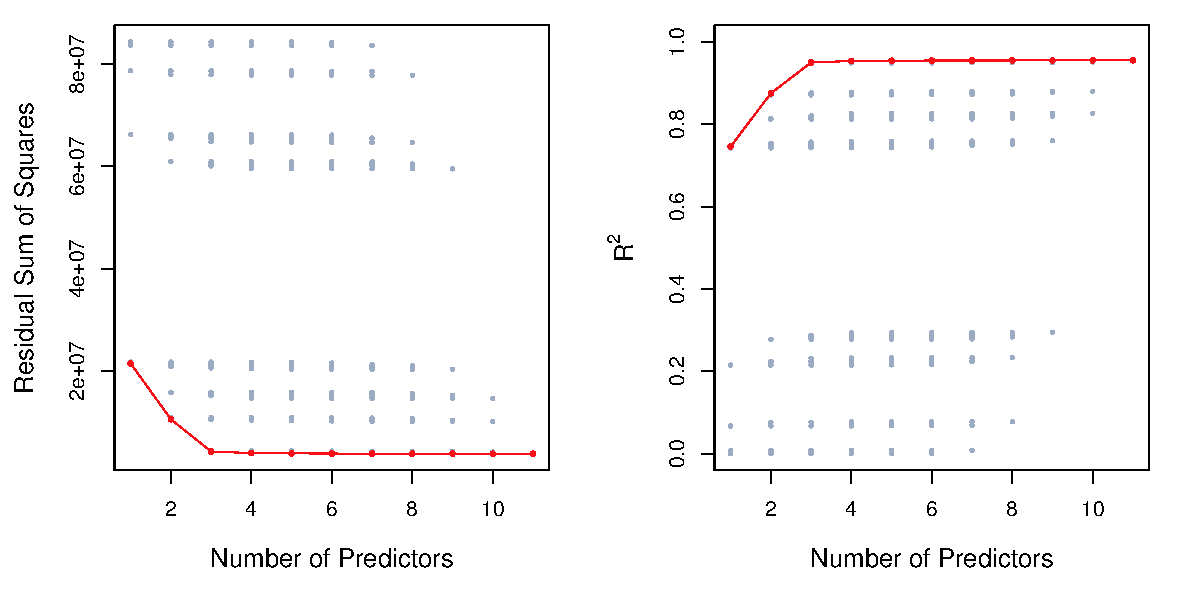
\includegraphics[width=0.92\textwidth,height=0.62\textheight,keepaspectratio]{6_1.pdf}
  \end{center}
  RSS, $R^2$, $C_p$, BIC, adjusted $R^2$ as $k$ varies. Note how
  different criteria can disagree on the optimal $k$.
  \islpsource{Figure 6.1}
\end{frame}

\begin{frame}{Forward stepwise selection}
  A greedy alternative when best subset is too expensive.
  \begin{block}{Algorithm}
    \begin{enumerate}
      \item Start with the null model $M_0$ (only intercept).
      \item For $k = 1, \ldots, p$: add to $M_{k-1}$ the predictor that
            most reduces RSS. Call the result $M_k$.
      \item Choose among $M_0, \ldots, M_p$ by CV / $C_p$ / BIC.
    \end{enumerate}
  \end{block}
  \begin{readme}
    Considers $1 + \sum_k (p - k) = O(p^2)$ models instead of $2^p$
    --- scales to large $p$. Greedy: not guaranteed to find the best
    subset.
  \end{readme}
\end{frame}

\begin{frame}{Backward and hybrid stepwise}
  \begin{columns}[T]
    \begin{column}{0.48\textwidth}
      \begin{block}{Backward}
        Start with the full model and drop the least useful predictor
        at each step. Requires $n > p$.
      \end{block}
    \end{column}
    \begin{column}{0.48\textwidth}
      \begin{block}{Hybrid}
        Alternate forward and backward steps. Recovers some of the
        flexibility of best subset at greedy cost.
      \end{block}
    \end{column}
  \end{columns}
  \begin{alertblock}{All three are heuristics}
    Forward, backward, and hybrid can disagree on the same data.
    Always cross-validate the chosen model.
  \end{alertblock}
\end{frame}

\begin{frame}{Best subset vs.\ forward stepwise: two search strategies}
  \begin{columns}[T]
    \begin{column}{0.5\textwidth}\centering
      {\small\textbf{Best subset: evaluate \emph{all} $2^p$}}\\[3pt]
      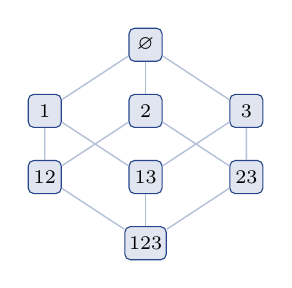
\begin{tikzpicture}[scale=0.8,every node/.style={font=\scriptsize},
          sub/.style={draw=accent,fill=accent!14,rounded corners=2pt,inner sep=1.5pt,minimum size=4.2mm}]
        \node[sub] (e) at (0,0) {$\varnothing$};
        \node[sub] (1) at (-1.6,-1.05) {$1$};
        \node[sub] (2) at (0,-1.05) {$2$};
        \node[sub] (3) at (1.6,-1.05) {$3$};
        \node[sub] (12) at (-1.6,-2.1) {$12$};
        \node[sub] (13) at (0,-2.1) {$13$};
        \node[sub] (23) at (1.6,-2.1) {$23$};
        \node[sub] (123) at (0,-3.15) {$123$};
        \foreach \a/\b in {e/1,e/2,e/3,1/12,1/13,2/12,2/23,3/13,3/23,12/123,13/123,23/123}
          \draw[accent!35,line width=0.5pt] (\a)--(\b);
      \end{tikzpicture}
    \end{column}
    \begin{column}{0.5\textwidth}\centering
      {\small\textbf{Forward: follow one greedy path}}\\[3pt]
      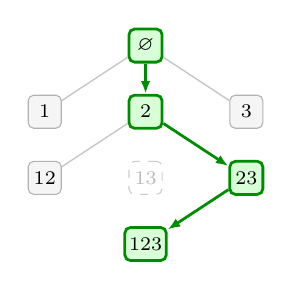
\begin{tikzpicture}[scale=0.8,every node/.style={font=\scriptsize},
          sub/.style={rounded corners=2pt,inner sep=1.5pt,minimum size=4.2mm},
          cand/.style={sub,draw=gray!60,fill=gray!8},
          pick/.style={sub,draw=green!55!black,fill=green!15,line width=1pt,font=\scriptsize\bfseries},
          skip/.style={sub,draw=gray!40,dashed,fill=none,text=gray!55}]
        \node[pick] (e) at (0,0) {$\varnothing$};
        \node[cand] (1) at (-1.6,-1.05) {$1$};
        \node[pick] (2) at (0,-1.05) {$2$};
        \node[cand] (3) at (1.6,-1.05) {$3$};
        \node[cand] (12) at (-1.6,-2.1) {$12$};
        \node[skip] (13) at (0,-2.1) {$13$};
        \node[pick] (23) at (1.6,-2.1) {$23$};
        \node[pick] (123) at (0,-3.15) {$123$};
        \draw[gray!45,line width=0.5pt] (e)--(1); \draw[gray!45,line width=0.5pt] (e)--(3);
        \draw[gray!45,line width=0.5pt] (2)--(12);
        \draw[-{Latex[length=1.6mm]},green!55!black,line width=1pt] (e)--(2);
        \draw[-{Latex[length=1.6mm]},green!55!black,line width=1pt] (2)--(23);
        \draw[-{Latex[length=1.6mm]},green!55!black,line width=1pt] (23)--(123);
      \end{tikzpicture}
    \end{column}
  \end{columns}
  \begin{takeaway}
    Best subset scores the \emph{whole} lattice ($2^p$ models); forward
    keeps only the winner at each level (green) and never even fits the
    dashed subset. At $p = 20$: $2^{20}\approx 10^6$ vs.\ $211$ models.
  \end{takeaway}
\end{frame}

\begin{frame}{Choosing $k$: four penalised criteria}
  Training RSS always decreases with $k$, so we need penalised
  criteria that approximate test error.
  \begin{block}{The four standard criteria}
    \begin{align*}
      C_p &= \tfrac{1}{n}\bigl(\mathrm{RSS} + 2 d \hat\sigma^2\bigr), \\
      \mathrm{AIC} &\propto C_p, \\
      \mathrm{BIC} &= \tfrac{1}{n}\bigl(\mathrm{RSS} + \log(n)\, d \hat\sigma^2\bigr), \\
      \mathrm{adj.}\,R^2 &= 1 - \tfrac{\mathrm{RSS}/(n - d - 1)}{\mathrm{TSS}/(n-1)}.
    \end{align*}
  \end{block}
  \begin{takeaway}
    All four share one shape --- \emph{training fit $+$ complexity
    penalty}; they differ only in how steeply each extra predictor is
    taxed.
  \end{takeaway}
\end{frame}

\begin{frame}{Reading the criteria symbol-by-symbol}
  \begin{readme}
    \begin{tabular}{@{}cl@{}}
      \toprule
      \textbf{Symbol} & \textbf{Meaning} \\
      \midrule
      $\mathrm{RSS}$ & Residual sum of squares (training fit) \\
      $d$ & Number of predictors in the model \\
      $\hat\sigma^2$ & Estimated noise variance \\
      $n$ & Sample size \\
      $\mathrm{TSS}$ & Total sum of squares \\
      \bottomrule
    \end{tabular}
  \end{readme}
  \begin{takeaway}[Practical guidance]
    BIC penalises more heavily for large $n$ $\Rightarrow$ smaller
    models. Use BIC when parsimony matters most. Cross-validation is
    more robust when distributional assumptions are uncertain.
  \end{takeaway}
\end{frame}

\begin{frame}{Exercise 6.1 --- Counting Models in Subset Selection [Math]}
  \begin{exercise}
    A regression problem has $p = 10$ candidate predictors.
    \begin{enumerate}
      \item How many models does \emph{best subset} selection consider
            in total (including the null model)? Give the general
            formula and the number.
      \item How many models does \emph{forward stepwise} selection fit
            in total? Give the general formula and the number.
      \item By roughly what factor does best subset exceed forward
            stepwise here, and why does the gap explode as $p$ grows?
    \end{enumerate}
  \end{exercise}
\end{frame}

\begin{frame}{Solution --- Exercise 6.1 (1/2)}
  \begin{solutionbox}
    \textbf{(1) Best subset.}
    For each size $k$ there are $\binom{p}{k}$ models, and summing over
    all sizes gives
    \[
      \sum_{k=0}^{p}\binom{p}{k} = 2^{p} .
    \]
    For $p = 10$: $\;2^{10} = 1024$ models.

    \textbf{(2) Forward stepwise.}
    Start from the null model, then at step $k$ (for
    $k = 0,\dots,p-1$) fit the $p - k$ models that add one predictor to
    the current model:
    \[
      1 + \sum_{k=0}^{p-1}(p-k) = 1 + \frac{p(p+1)}{2} .
    \]
    For $p = 10$: $\;1 + \tfrac{10\cdot 11}{2} = 1 + 55 = 56$ models.
    (Backward stepwise fits the same count, $O(p^2)$.)
  \end{solutionbox}
\end{frame}

\begin{frame}{Solution --- Exercise 6.1 (2/2)}
  \begin{solutionbox}
    \textbf{(3) The gap.}
    Here $1024 / 56 \approx 18\times$. Best subset grows
    \emph{exponentially} ($2^p$) while forward stepwise grows only
    \emph{quadratically} ($O(p^2)$). For $p = 20$, best subset already
    considers $2^{20} \approx 10^6$ models versus
    $1 + \tfrac{20 \cdot 21}{2} = 211$ for forward stepwise --- which is
    why best subset is infeasible beyond $p \approx 30$ and stepwise
    heuristics are used instead.

    \emph{Interpretation.} The saving is bought with greed: forward
    stepwise commits to one predictor per step and walks a single path
    through the model lattice, so it can miss the best subset of a given
    size --- its winner must still be validated by CV or a penalised
    criterion.

    \emph{Common mistake:} dropping the null model from either count ---
    both include it ($2^{10} = 1024$ subsets \emph{including}
    $\varnothing$; $1 + 55 = 56$ stepwise fits, the leading $1$ being
    $M_0$).
  \end{solutionbox}
\end{frame}

\begin{frame}{Exercise 6.2 --- Why RSS and $R^2$ Cannot Pick the Size [Concept]}
  \begin{exercise}
    \begin{enumerate}
      \item Explain why training RSS and training $R^2$ can never be
            used to choose the \emph{number} of predictors $d$.
      \item What quantity do $C_p$, AIC, and BIC try to estimate that
            training RSS does not?
      \item State qualitatively how $C_p$, BIC, and adjusted $R^2$
            modify the raw training fit, and which of them most favours
            small models.
    \end{enumerate}
  \end{exercise}
\end{frame}

\begin{frame}{Solution --- Exercise 6.2}
  \begin{solutionbox}
    \textbf{(1) Monotonicity.}
    Adding a predictor to a nested least-squares model can never
    increase RSS (the extra coefficient can always be set to zero), so
    RSS is \emph{non-increasing} in $d$ and $R^2 = 1 - \mathrm{RSS}/
    \mathrm{TSS}$ is \emph{non-decreasing}. Both are therefore optimised
    by the largest model, giving no guidance on size and rewarding
    overfitting.

    \textbf{(2) What the criteria estimate.}
    They estimate the \emph{test} error (expected prediction error on
    new data), not the training error. Each adds a penalty that grows
    with $d$ to counteract the optimism of the training fit.

    \textbf{(3) How they adjust the fit.}
    \begin{itemize}
      \item $C_p = \tfrac1n(\mathrm{RSS} + 2 d\hat\sigma^2)$: adds a
            penalty $2d\hat\sigma^2$ (AIC is proportional to it).
      \item $\mathrm{BIC} = \tfrac1n(\mathrm{RSS} + \log(n)\,
            d\hat\sigma^2)$: same shape but penalty $\log(n)\,
            d\hat\sigma^2$. Since $\log n > 2$ for $n > 7$, BIC
            penalises extra predictors more heavily and therefore
            \emph{most favours small (parsimonious) models}.
      \item Adjusted $R^2 = 1 - \tfrac{\mathrm{RSS}/(n-d-1)}
            {\mathrm{TSS}/(n-1)}$: divides RSS by its degrees of
            freedom, so it can \emph{decrease} when a useless predictor
            is added.
    \end{itemize}
    We pick the model that minimises $C_p$/AIC/BIC or maximises
    adjusted $R^2$.
  \end{solutionbox}
\end{frame}

\begin{frame}{Exercise 6.3 --- Computing $C_p$ and BIC [Math]}
  \begin{exercise}
    With $n = 100$ observations and $\hat\sigma^2 = 4$, two candidate
    models give:
    \begin{center}
      \begin{tabular}{lcc}
        \toprule
        & $d$ & RSS \\
        \midrule
        Model A & $3$ & $480$ \\
        Model B & $6$ & $450$ \\
        \bottomrule
      \end{tabular}
    \end{center}
    Compute $C_p$ and BIC for each model and state which model each
    criterion selects. Use
    $C_p = \tfrac1n(\mathrm{RSS} + 2 d\hat\sigma^2)$ and
    $\mathrm{BIC} = \tfrac1n(\mathrm{RSS} + \log(n)\, d\hat\sigma^2)$.
  \end{exercise}
\end{frame}

\begin{frame}{Solution --- Exercise 6.3 (1/2)}
  \begin{solutionbox}
    Here $n = 100$, $\hat\sigma^2 = 4$, and $\log(100) \approx 4.605$.
    Both criteria share the shape $\tfrac1n(\mathrm{RSS} +
    \text{price} \times d\hat\sigma^2)$; only the per-predictor price
    differs ($2$ for $C_p$ vs.\ $\log n$ for BIC).

    \textbf{$C_p$} (price $2$ per predictor).
    \begin{align*}
      C_p^A &= \tfrac{1}{100}\bigl(480 + 2\cdot 3\cdot 4\bigr)
             = \tfrac{1}{100}(480 + 24) = 5.04 , \\
      C_p^B &= \tfrac{1}{100}\bigl(450 + 2\cdot 6\cdot 4\bigr)
             = \tfrac{1}{100}(450 + 48) = 4.98 .
    \end{align*}
    $C_p$ is smaller for \textbf{Model B} ($4.98 < 5.04$), so $C_p$
    selects B: B's RSS saving of $480 - 450 = 30$ outweighs its extra
    penalty of $48 - 24 = 24$.
  \end{solutionbox}
\end{frame}

\begin{frame}{Solution --- Exercise 6.3 (2/2)}
  \begin{solutionbox}
    \textbf{BIC} (price $\log(100) \approx 4.605$ per predictor).
    \begin{align*}
      \mathrm{BIC}^A &= \tfrac{1}{100}\bigl(480 + 4.605\cdot 3\cdot 4\bigr)
             = \tfrac{1}{100}(480 + 55.3) = 5.353 , \\
      \mathrm{BIC}^B &= \tfrac{1}{100}\bigl(450 + 4.605\cdot 6\cdot 4\bigr)
             = \tfrac{1}{100}(450 + 110.5) = 5.605 .
    \end{align*}
    BIC is smaller for \textbf{Model A} ($5.353 < 5.605$), so BIC
    selects A: the same RSS saving of $30$ must now beat an extra
    penalty of $110.5 - 55.3 = 55.2$ --- and fails.

    \textbf{Interpretation.}
    The two criteria disagree: BIC's heavier $\log(n)$ penalty punishes
    the three extra predictors of Model B more than they reduce RSS, so
    BIC prefers the smaller Model A, while the lighter $C_p$ penalty
    lets Model B's better fit win. When parsimony matters, follow BIC.

    \emph{Common mistake:} using $\log_{10}(100) = 2$ instead of the
    natural log $\ln(100) \approx 4.605$ --- with base-$10$ logs the BIC
    penalty would collapse to $C_p$'s $2d\hat\sigma^2$ here.
  \end{solutionbox}
\end{frame}


\begin{frame}{Choosing the model size: $C_p$, BIC and adjusted $R^2$}
  \begin{center}
    
\includegraphics[width=0.98\textwidth,height=0.56\textheight,keepaspectratio]{ch06_selection_criteria.png}
  \end{center}
  \begin{takeaway}Each criterion trades goodness-of-fit against complexity; BIC's heavier penalty picks the smallest model, $C_p$ and adjusted $R^2$ a slightly larger one.\end{takeaway}
\end{frame}

\begin{frame}{Extended Exercise 6.1 --- $C_p$, BIC and Adjusted $R^2$ Across Sizes [Math]}
  \begin{longexercise}
    Best-subset selection on a problem with $n=100$ and $p=4$ returns the
    best model of each size, with residual sums of squares (and
    $\hat\sigma^2=5$ estimated from the full model):
    \begin{center}\footnotesize
      \begin{tabular}{lccccc}
        \toprule
        $d$ & $0$ & $1$ & $2$ & $3$ & $4$ \\
        \midrule
        RSS & $900$ & $500$ & $340$ & $322$ & $314$ \\
        \bottomrule
      \end{tabular}
    \end{center}
    \begin{enumerate}
      \item Compute $C_p$, BIC and adjusted $R^2$ for each size, using
            $C_p=\tfrac1n(\mathrm{RSS}+2d\hat\sigma^2)$,
            $\mathrm{BIC}=\tfrac1n(\mathrm{RSS}+\log(n)d\hat\sigma^2)$ and
            $\mathrm{adj}\,R^2=1-\tfrac{\mathrm{RSS}/(n-d-1)}
            {\mathrm{TSS}/(n-1)}$ with $\mathrm{TSS}=\mathrm{RSS}_{d=0}$.
      \item State the winner under each criterion and explain any
            disagreement.
      \item How many models did best subset examine, and how many would
            forward stepwise fit?
    \end{enumerate}
  \end{longexercise}
\end{frame}

\begin{frame}{Solution --- Extended Exercise 6.1 (1/3)}
  \begin{solutionbox}
    With $n=100$, $\hat\sigma^2=5$ and $\log(100)\approx4.605$, the
    per-parameter penalties are $2\hat\sigma^2=10$ ($C_p$) and
    $\log(n)\hat\sigma^2\approx23.03$ (BIC). Dividing by $n=100$:
    \[\footnotesize
      \begin{array}{c|ccccc}
        d & 0 & 1 & 2 & 3 & 4\\\hline
        C_p          & 9.00 & 5.10 & 3.60 & \mathbf{3.52} & 3.54\\[1pt]
        \mathrm{BIC} & 9.00 & 5.23 & \mathbf{3.86} & 3.91 & 4.06
      \end{array}
    \]
    For example $C_p(3)=\tfrac1{100}(322+2\cdot3\cdot5)=\tfrac{352}{100}
    =3.52$ and $\mathrm{BIC}(2)=\tfrac1{100}(340+4.605\cdot2\cdot5)
    =\tfrac{386.05}{100}=3.86$.
  \end{solutionbox}
\end{frame}

\begin{frame}{Solution --- Extended Exercise 6.1 (2/3)}
  \begin{solutionbox}
    \textbf{Adjusted $R^2$} with $\mathrm{TSS}=900$ and
    $\mathrm{TSS}/(n-1)=900/99=9.09$:
    \[\footnotesize
      \begin{array}{c|ccccc}
        d & 0 & 1 & 2 & 3 & 4\\\hline
        \mathrm{RSS}/(n\!-\!d\!-\!1) & 9.09 & 5.10 & 3.51 & 3.35 & 3.31\\[1pt]
        \mathrm{adj}\,R^2 & 0.00 & 0.44 & 0.61 & 0.63 & \mathbf{0.636}
      \end{array}
    \]
    e.g.\ at $d=4$: $1-\tfrac{314/95}{900/99}=1-\tfrac{3.305}{9.091}
    =0.636$.

    \textbf{Winners.} $C_p\Rightarrow d=3$;\quad
    $\mathrm{BIC}\Rightarrow d=2$;\quad
    $\mathrm{adj}\,R^2\Rightarrow d=4$.

    \emph{Common mistake:} dividing by $n - d$ instead of $n - d - 1$ in
    the numerator --- the extra $-1$ is the intercept. At $d = 4$ the
    correct divisor is $95$, not $96$: $314/95 = 3.305$.
  \end{solutionbox}
\end{frame}

\begin{frame}{Solution --- Extended Exercise 6.1 (3/3)}
  \begin{solutionbox}
    \textbf{(2) Why they disagree.} All three add a complexity penalty
    to the training fit, but with different strengths. BIC's penalty
    $\log(n)\approx4.6$ per parameter is heaviest, so it stops earliest
    at the parsimonious $d=2$. $C_p$/AIC use the lighter penalty $2$, so
    they tolerate the small RSS drop $340\!\to\!322$ and pick $d=3$.
    Adjusted $R^2$ penalises size only mildly and keeps improving to
    $d=4$. Ordering by aggressiveness of shrinkage in model size,
    $\mathrm{BIC}\le C_p\le\mathrm{adj}\,R^2$ --- exactly the pattern in
    Figure~6.1.

    \textbf{(3) Search cost.} Best subset examines $2^p=2^4=16$ models;
    forward stepwise fits $1+\tfrac{p(p+1)}2=1+10=11$. The gap is tiny
    here but explodes with $p$: at $p=20$ it is $2^{20}\approx10^6$
    versus $211$ --- why best subset is infeasible past $p\approx30$.
  \end{solutionbox}
\end{frame}

% ============================================================
\section{Ridge regression}
% ============================================================

\begin{frame}{Why ridge: numerical stability via a penalty}
  Subset selection is discrete and combinatorial. A smoother
  alternative: keep all predictors but penalise large coefficients.
  \begin{takeaway}[Intuition]
    The penalty pulls $\hat\beta$ toward zero, especially when the
    data don't strongly constrain it. We trade a small upward bias
    for a large reduction in variance.
  \end{takeaway}
  \begin{readme}
    Two payoffs at once: the penalty (i) \emph{stabilises} the fit when
    predictors are collinear, and (ii) \emph{lowers variance} by
    refusing to chase noise with large coefficients.
  \end{readme}
\end{frame}

\begin{frame}{The ridge regression objective}
  \begin{block}{Objective}
    \[
      \boxed{\;
        \hat\beta^{\,\mathrm R} = \arg\min_{\beta}
        \biggl\{ \underbrace{\sum_{i=1}^n (y_i - \beta_0 - X_i^\top\beta)^2}_{\mathrm{RSS}}
                + \underbrace{\lambda \sum_{j=1}^p \beta_j^2}_{\ell_2 \text{ penalty}} \biggr\}.
      \;}
    \]
  \end{block}
  \begin{takeaway}
    Minimise training error \emph{plus} a size tax on the coefficients;
    the tuning parameter $\lambda$ sets how hard we pull them toward
    zero.
  \end{takeaway}
\end{frame}

\begin{frame}{Reading the ridge objective}
  \begin{readme}
    \begin{tabular}{@{}cl@{}}
      \toprule
      \textbf{Term} & \textbf{Role} \\
      \midrule
      RSS & Training fit: pulls coefficients toward the OLS solution. \\
      $\lambda \sum \beta_j^2$ & Penalty: pulls coefficients toward zero. \\
      $\lambda$ & Tuning parameter that controls the trade-off. \\
      \bottomrule
    \end{tabular}
  \end{readme}
  \begin{itemize}
    \item $\lambda = 0$ recovers ordinary least squares.
    \item $\lambda \to \infty$ drives every $\hat\beta^{\,\mathrm R} \to 0$.
    \item Closed form:
          $\hat\beta^{\,\mathrm R} = (\mathbf{X}^\top \mathbf{X} + \lambda I)^{-1}\mathbf{X}^\top \mathbf{y}$.
  \end{itemize}
\end{frame}

\begin{frame}{Three ways to think about ridge}
  \begin{block}{Numerical stability}
    Adding $\lambda I$ stabilises the inverse when
    $\mathbf{X}^\top\mathbf{X}$ is near-singular (collinearity).
  \end{block}
  \begin{block}{Bias-variance trade-off}
    Trades a small upward bias for a large reduction in variance.
    Especially helpful when $p$ is large relative to $n$.
  \end{block}
  \begin{alertblock}{Standardise first!}
    The penalty is not scale-invariant. Standardise predictors before
    fitting, otherwise ridge will preferentially shrink variables with
    larger units.
  \end{alertblock}
\end{frame}

\begin{frame}{Ridge's bias-variance trade-off, visualised}
  \begin{center}
    
\includegraphics[width=0.84\textwidth,height=0.52\textheight,keepaspectratio]{ch06_ridge_bias_variance.png}
  \end{center}
  \begin{takeaway}
    As $\lambda$ grows, variance falls but squared bias rises. Test
    error is their sum plus the irreducible $\sigma^2$, so it bottoms
    out at an \emph{intermediate} $\lambda$ --- the one cross-validation
    aims to find.
  \end{takeaway}
\end{frame}

\begin{frame}{Ridge: coefficient paths}
  \begin{center}
    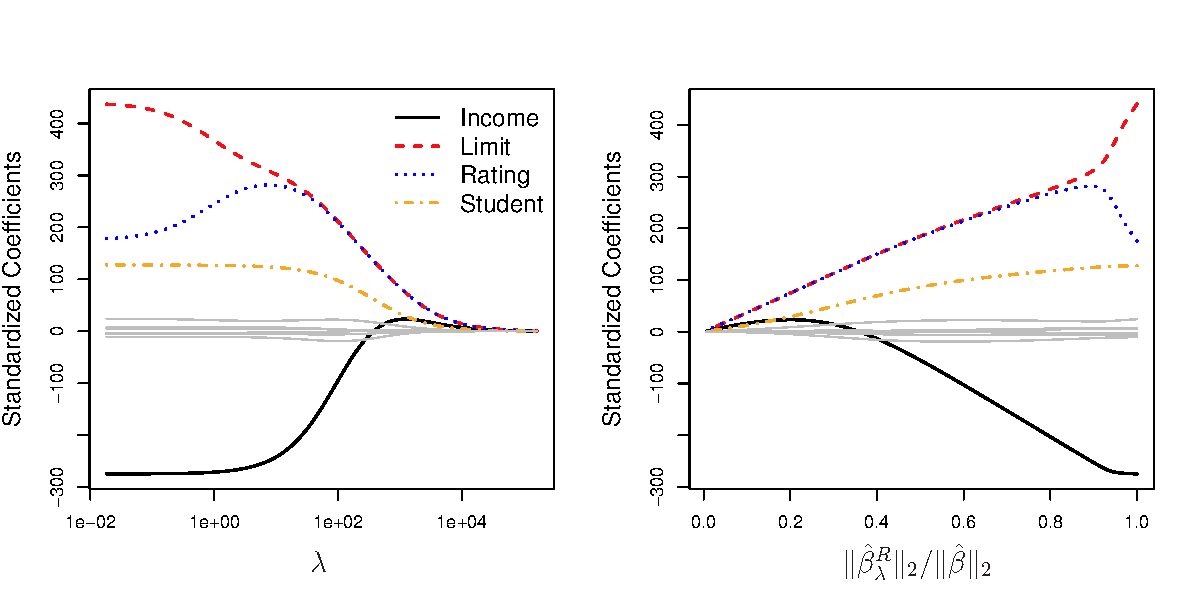
\includegraphics[width=0.85\textwidth,height=0.62\textheight,keepaspectratio]{6_4.pdf}
  \end{center}
  Each line is one $\hat\beta_j$ as $\lambda$ grows from left to right.
  Coefficients shrink smoothly toward zero --- but never exactly reach
  zero.
  \islpsource{Figure 6.4}
\end{frame}

\begin{frame}{Exercise 6.4 --- Ridge: $\lambda$ and Standardisation [Concept]}
  \begin{exercise}
    \begin{enumerate}
      \item Describe what happens to the ridge coefficients
            $\hat\beta^{\,\mathrm R}$ as $\lambda$ increases from $0$ to
            $\infty$, and to the model's bias and variance.
      \item Why must predictors be standardised before ridge regression?
            What goes wrong if one predictor is measured in metres and
            another in millimetres?
      \item Does ridge ever set a coefficient exactly to zero? What does
            this imply for interpretability?
    \end{enumerate}
  \end{exercise}
\end{frame}

\begin{frame}{Solution --- Exercise 6.4}
  \begin{solutionbox}
    \textbf{(1) Effect of $\lambda$.}
    At $\lambda = 0$ ridge equals OLS. As $\lambda$ grows the $\ell_2$
    penalty pulls all coefficients smoothly toward zero, and as
    $\lambda \to \infty$ every $\hat\beta_j^{\,\mathrm R} \to 0$ (only
    the intercept survives). Increasing $\lambda$ \emph{increases bias}
    (the fit is pulled away from the data) but \emph{decreases variance}
    (the coefficients become more stable). The best $\lambda$, chosen by
    cross-validation, trades a little bias for a large variance
    reduction.

    \textbf{(2) Why standardise.}
    The penalty $\lambda\sum_j \beta_j^2$ is \emph{not scale invariant}.
    A predictor measured in millimetres has a coefficient $1000\times$
    larger than the same predictor in metres, so it would be penalised
    $10^6$ times more heavily and shrunk far more aggressively --- an
    arbitrary artefact of units, not of importance. Standardising each
    predictor to unit variance (typically $\tilde x_{ij} = x_{ij}/
    \hat\sigma_j$) puts them on a common footing so the penalty treats
    them comparably.

    \textbf{(3) No exact zeros.}
    Ridge shrinks coefficients toward zero but essentially never sets
    them \emph{exactly} to zero (the $\ell_2$ penalty is smooth at the
    origin). So ridge keeps all $p$ predictors in the model; it improves
    prediction and stability but does \emph{not} perform variable
    selection --- for that, use the lasso.
  \end{solutionbox}
\end{frame}


\begin{frame}{Ridge coefficient paths on Hitters}
  \begin{center}
    
\includegraphics[width=0.82\textwidth,height=0.58\textheight,keepaspectratio]{ch06_ridge_path.png}
  \end{center}
  \begin{takeaway}As $\lambda$ grows every coefficient shrinks smoothly toward zero, but none is set \emph{exactly} to zero --- ridge keeps all predictors.\end{takeaway}
\end{frame}

\begin{frame}{Choosing $\lambda$ by cross-validation on Hitters}
  \begin{center}
\includegraphics[width=0.88\textwidth,height=0.56\textheight,keepaspectratio]{ch06_x_ridge_cv.png}\end{center}
  \begin{takeaway}The 10-fold CV curve on standardised Hitters dips at $\lambda^*\approx 1.6$ (CV MSE $\approx 114{,}000$) --- mild shrinkage beats OLS, and the error climbs steeply once heavy shrinkage drowns the signal.\end{takeaway}
\end{frame}

% ============================================================
\section{The Lasso}
% ============================================================

\begin{frame}{The lasso: change the penalty, change the behaviour}
  Same idea as ridge but with an $\ell_1$ penalty instead of $\ell_2$.
  \begin{block}{Objective}
    \[
      \boxed{\;
        \hat\beta^{\,\mathrm L} = \arg\min_{\beta}
        \biggl\{ \mathrm{RSS} + \lambda \sum_{j=1}^p |\beta_j| \biggr\}.
      \;}
    \]
  \end{block}
  \begin{readme}
    The \emph{only} change from ridge is $|\beta_j|$ in place of
    $\beta_j^2$ --- and that kink at the origin is exactly what lets
    coefficients reach zero.
  \end{readme}
  \begin{takeaway}[The crucial property]
    For $\lambda$ large enough, some $\hat\beta_j^{\,\mathrm L} = 0$
    \emph{exactly}. The lasso \emph{performs variable selection}
    automatically as a side effect of fitting.
  \end{takeaway}
\end{frame}

\begin{frame}{Lasso: coefficient paths}
  \begin{center}
    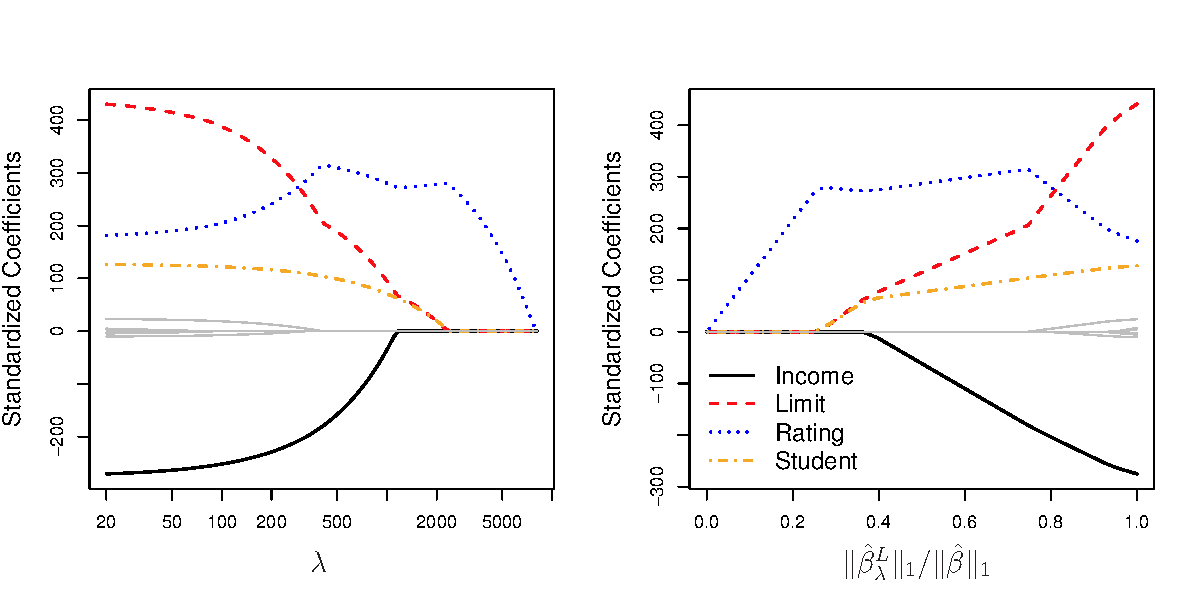
\includegraphics[width=0.85\textwidth,height=0.62\textheight,keepaspectratio]{6_6.pdf}
  \end{center}
  As $\lambda$ grows, coefficients hit zero one by one. The lasso
  delivers a continuum of sparse models indexed by $\lambda$.
  \islpsource{Figure 6.6}
\end{frame}

\begin{frame}{Why does lasso produce zeros? --- the geometry}
  \begin{columns}[T]
    \begin{column}{0.55\textwidth}
      \begin{block}{The unit balls}
        \begin{itemize}
          \item Ridge constrains $\sum \beta_j^2 \le t$ --- a smooth
                ball.
          \item Lasso constrains $\sum |\beta_j| \le t$ --- a polytope
                with corners on the axes.
        \end{itemize}
      \end{block}
      \begin{takeaway}
        The level sets of the squared-error loss are likely to first
        touch the lasso ball at a corner --- a corner has some
        $\beta_j = 0$.
      \end{takeaway}
    \end{column}
    \begin{column}{0.42\textwidth}
      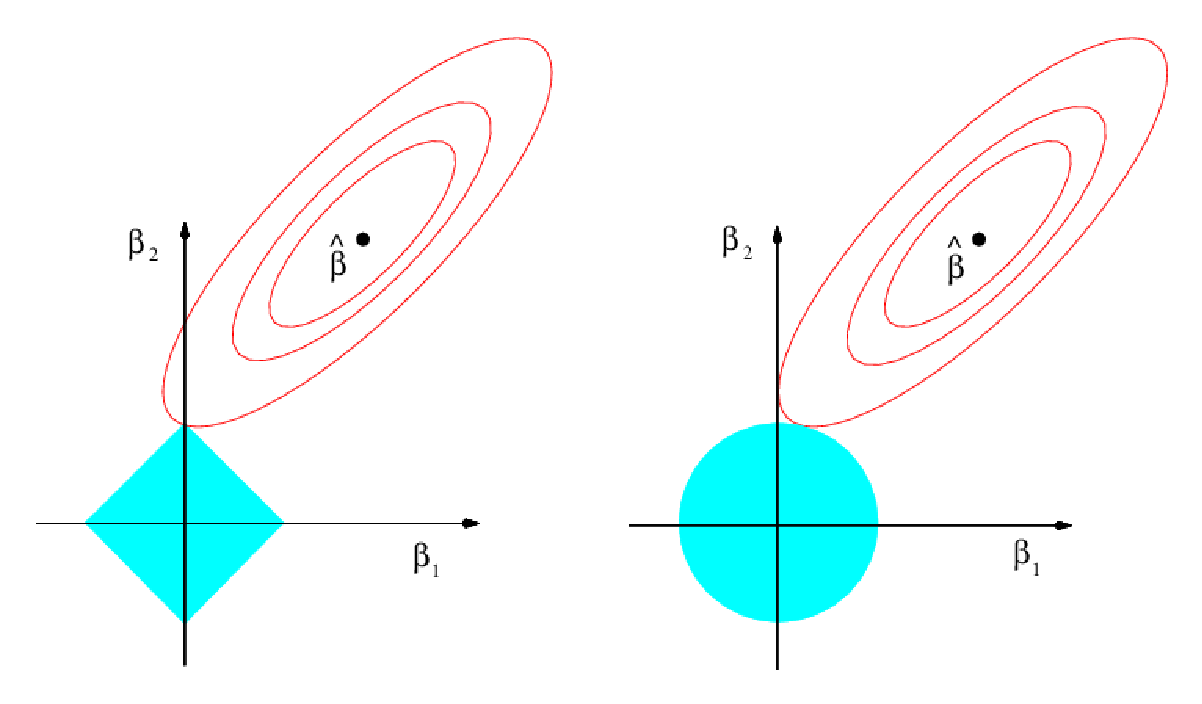
\includegraphics[width=\textwidth,height=0.55\textheight,keepaspectratio]{6_7.pdf}
    \end{column}
  \end{columns}
  \islpsource{Figure 6.7}
\end{frame}

\begin{frame}{Choose $\lambda$ by cross-validation}
  Both ridge and lasso introduce a single tuning parameter.
  \begin{block}{The procedure}
    \begin{enumerate}
      \item Run $k$-fold CV over a logarithmic grid of $\lambda$
            values (say, $50$ from $10^{-3}$ to $10^3$).
      \item Pick the $\lambda$ that minimises CV error, or apply the
            \emph{one-standard-error rule}: the largest $\lambda$
            within one standard error of the minimum.
      \item Re-fit on the full data at that $\lambda$.
    \end{enumerate}
  \end{block}
  \begin{readme}
    In Python: \texttt{sklearn.linear\_model.RidgeCV} and
    \texttt{LassoCV} perform the grid search internally.
  \end{readme}
\end{frame}

\begin{frame}{Ridge vs.\ lasso vs.\ elastic net: when each wins}
  \begin{columns}[T]
    \begin{column}{0.32\textwidth}
      \begin{block}{Ridge}
        Many small effects, none dominant. Predictors all somewhat
        useful.
      \end{block}
    \end{column}
    \begin{column}{0.32\textwidth}
      \begin{block}{Lasso}
        Truth is sparse: a few predictors carry the signal, the rest
        are noise.
      \end{block}
    \end{column}
    \begin{column}{0.32\textwidth}
      \begin{block}{Elastic net}
        $\alpha\|\beta\|_1 + (1-\alpha)\|\beta\|_2^2$. Useful for
        sparse + correlated predictors.
      \end{block}
    \end{column}
  \end{columns}
  \begin{takeaway}[Default workflow]
    Try lasso first. If you see correlated predictors splitting their
    estimated effects, fall back to elastic net or ridge.
  \end{takeaway}
\end{frame}


\begin{frame}{Mini-check: ridge vs.\ lasso}
  \begin{readme}[Quick self-assessment]
    For each scenario, which method is more appropriate?
    \begin{enumerate}
      \item Many predictors, all expected to have small effects.
      \item Truth is sparse: only a handful of predictors matter.
      \item Severe multicollinearity, want a stable fit.
      \item Want automatic variable selection.
    \end{enumerate}
  \end{readme}
  \begin{takeaway}[Answers]
    1.\ Ridge.\quad 2.\ Lasso.\quad 3.\ Ridge.\quad 4.\ Lasso (or elastic
    net).
  \end{takeaway}
\end{frame}

\begin{frame}{Exercise 6.5 --- Lasso Sparsity: $\ell_1$ vs.\ $\ell_2$ [Concept/Math]}
  \begin{exercise}
    \begin{enumerate}
      \item Write the constrained (budget) form of ridge and lasso and
            describe the shape of each constraint region in two
            dimensions.
      \item Use that geometry to explain why the lasso produces exact
            zeros while ridge does not.
      \item \emph{Orthonormal design.} When
            $\mathbf{X}^\top\mathbf{X} = I$, the lasso has the
            closed-form soft-threshold solution
            $\hat\beta_j^{\,\mathrm L} =
            \mathrm{sign}(\hat\beta_j^{\,\mathrm{OLS}})
            \bigl(|\hat\beta_j^{\,\mathrm{OLS}}| - \lambda/2\bigr)_{+}$.
            If $\hat\beta_j^{\,\mathrm{OLS}} = 1.5$ and $\lambda = 4$,
            compute $\hat\beta_j^{\,\mathrm L}$.
    \end{enumerate}
  \end{exercise}
\end{frame}

\begin{frame}{Solution --- Exercise 6.5 (1/2)}
  \begin{solutionbox}
    \textbf{(1) Constraint regions.}
    Both methods can be written as minimise RSS subject to a budget:
    \[
      \text{ridge: } \sum_j \beta_j^2 \le t,
      \qquad
      \text{lasso: } \sum_j |\beta_j| \le t .
    \]
    In two dimensions the ridge region is a \emph{disc} (smooth,
    rounded), while the lasso region is a \emph{diamond} (a square
    rotated $45^\circ$) with sharp corners lying on the coordinate axes.

    \textbf{(2) Why lasso gives zeros.}
    The elliptical contours of the RSS expand until they first touch the
    constraint region; the solution is that contact point. The lasso
    diamond has corners \emph{on the axes}, where one coordinate is
    exactly zero, and contours are very likely to hit a corner first ---
    yielding $\hat\beta_j = 0$. The ridge disc has no corners, so the
    contact point almost never lands exactly on an axis; ridge shrinks
    but does not zero out. This is why the $\ell_1$ penalty performs
    variable selection and the $\ell_2$ penalty does not.
  \end{solutionbox}
\end{frame}

\begin{frame}{Solution --- Exercise 6.5 (2/2)}
  \begin{solutionbox}
    \textbf{(3) Soft-thresholding.}
    With $\hat\beta_j^{\,\mathrm{OLS}} = 1.5$ and $\lambda = 4$:
    \[
      |\hat\beta_j^{\,\mathrm{OLS}}| - \lambda/2 = 1.5 - 2.0 = -0.5 < 0 ,
    \]
    so $(\,\cdot\,)_{+} = 0$ and $\hat\beta_j^{\,\mathrm L} = 0$: the
    predictor is dropped. Had $\lambda = 2$ instead, we would get
    $\mathrm{sign}(1.5)(1.5 - 1.0) = +0.5$ --- shrunk toward zero but
    retained. This shows algebraically how the lasso zeros out
    coefficients once the penalty exceeds twice the OLS magnitude, while
    the ridge solution $\hat\beta_j/(1+\lambda)$ would only shrink,
    never reaching zero.

    \emph{Common mistake:} thresholding at $\lambda$ instead of
    $\lambda/2$. Here both give zero, but at $\lambda = 2$ the wrong
    threshold yields $1.5 - 2 < 0 \Rightarrow 0$, killing a coefficient
    that actually survives as $1.5 - 1.0 = 0.5$.
  \end{solutionbox}
\end{frame}

\begin{frame}{Lasso coefficient paths on Hitters}
  \begin{center}
    
\includegraphics[width=0.82\textwidth,height=0.58\textheight,keepaspectratio]{ch06_lasso_path.png}
  \end{center}
  \begin{takeaway}Unlike ridge, the lasso drives coefficients to \emph{exactly} zero as $\lambda$ grows --- it performs automatic variable selection.\end{takeaway}
\end{frame}

\begin{frame}{Why the lasso is sparse: the constraint geometry}
  \begin{columns}[c]
    \begin{column}{0.5\textwidth}\centering
      {\small\textbf{Lasso ($\ell_1$ diamond)}}\\[3pt]
      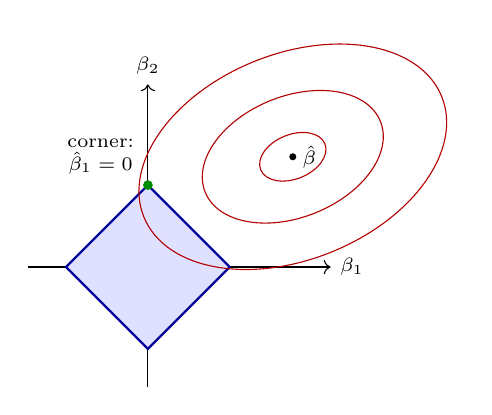
\begin{tikzpicture}[scale=0.8]
        \draw[->] (-1.9,0)--(2.9,0) node[right,font=\scriptsize]{$\beta_1$};
        \draw[->] (0,-1.9)--(0,2.9) node[above,font=\scriptsize]{$\beta_2$};
        \fill[blue!12,draw=blue!60!black,line width=0.8pt] (1.3,0)--(0,1.3)--(-1.3,0)--(0,-1.3)--cycle;
        \foreach \r in {0.55,1.5,2.55}{\draw[red!70!black,rotate around={22:(2.3,1.75)}] (2.3,1.75) ellipse [x radius=\r, y radius=0.64*\r];}
        \fill (2.3,1.75) circle (1.6pt) node[right,font=\scriptsize]{$\hat\beta$};
        \fill[green!55!black] (0,1.3) circle (2.2pt);
        \node[font=\scriptsize,align=center] at (-0.75,1.75) {corner:\\$\hat\beta_1=0$};
      \end{tikzpicture}
    \end{column}
    \begin{column}{0.5\textwidth}\centering
      {\small\textbf{Ridge ($\ell_2$ circle)}}\\[3pt]
      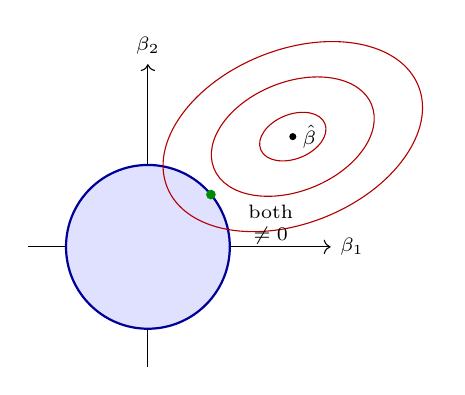
\begin{tikzpicture}[scale=0.8]
        \draw[->] (-1.9,0)--(2.9,0) node[right,font=\scriptsize]{$\beta_1$};
        \draw[->] (0,-1.9)--(0,2.9) node[above,font=\scriptsize]{$\beta_2$};
        \fill[blue!12,draw=blue!60!black,line width=0.8pt] (0,0) circle (1.3);
        \foreach \r in {0.55,1.35,2.15}{\draw[red!70!black,rotate around={22:(2.3,1.75)}] (2.3,1.75) ellipse [x radius=\r, y radius=0.64*\r];}
        \fill (2.3,1.75) circle (1.6pt) node[right,font=\scriptsize]{$\hat\beta$};
        \fill[green!55!black] (1.0,0.83) circle (2.2pt);
        \node[font=\scriptsize,align=center] at (1.95,0.35) {both\\$\ne 0$};
      \end{tikzpicture}
    \end{column}
  \end{columns}
  \begin{takeaway}RSS contours first touch the $\ell_1$ diamond at a \emph{corner} ($\hat\beta_j=0$); the smooth $\ell_2$ circle almost never does.\end{takeaway}
\end{frame}

\begin{frame}{Extended Exercise 6.2 --- Orthonormal Design: Ridge vs.\ Lasso [Math]}
  \begin{longexercise}
    Assume an \emph{orthonormal} design, $\mathbf{X}^\top\mathbf{X}=I$,
    so the OLS estimates are $\hat\beta_j^{\mathrm{OLS}}
    =(\mathbf{X}^\top\mathbf{y})_j$ and the objective separates
    coordinate-by-coordinate.
    \begin{enumerate}
      \item \textbf{Ridge.} Minimise
            $\lVert\mathbf{y}-\mathbf{X}\beta\rVert^2+\lambda
            \lVert\beta\rVert_2^2$ and show
            $\hat\beta_j^{\mathrm R}=\hat\beta_j^{\mathrm{OLS}}/(1+\lambda)$.
      \item \textbf{Lasso.} Minimise
            $\lVert\mathbf{y}-\mathbf{X}\beta\rVert^2+\lambda
            \lVert\beta\rVert_1$ and derive the soft-threshold solution
            $\hat\beta_j^{\mathrm L}
            =\mathrm{sign}(\hat\beta_j^{\mathrm{OLS}})
            \bigl(|\hat\beta_j^{\mathrm{OLS}}|-\lambda/2\bigr)_+$.
      \item \textbf{Apply} both with $\lambda=1$ to
            $\hat\beta^{\mathrm{OLS}}=(3.0,\,-1.5,\,0.4,\,-0.2)$ and
            comment on shrinkage vs.\ selection.
    \end{enumerate}
  \end{longexercise}
\end{frame}

\begin{frame}{Solution --- Extended Exercise 6.2 (1/2)}
  \begin{solutionbox}
    Because $\mathbf{X}^\top\mathbf{X}=I$,
    $\lVert\mathbf{y}-\mathbf{X}\beta\rVert^2=\text{const}
    +\sum_j\bigl(\beta_j-\hat\beta_j^{\mathrm{OLS}}\bigr)^2$, so every
    penalty separates across $j$.

    \textbf{(1) Ridge.} Minimise
    $(\beta_j-\hat\beta_j^{\mathrm{OLS}})^2+\lambda\beta_j^2$. Setting the
    derivative to zero,
    $2(\beta_j-\hat\beta_j^{\mathrm{OLS}})+2\lambda\beta_j=0
    \Rightarrow(1+\lambda)\beta_j=\hat\beta_j^{\mathrm{OLS}}$, hence
    $\boxed{\hat\beta_j^{\mathrm R}=\hat\beta_j^{\mathrm{OLS}}/(1+\lambda)}$
    --- a constant \emph{shrinkage factor}, never exactly zero.

    \textbf{(2) Lasso.} Minimise
    $(\beta_j-\hat\beta_j^{\mathrm{OLS}})^2+\lambda|\beta_j|$. For
    $\beta_j>0$, $2(\beta_j-\hat\beta_j^{\mathrm{OLS}})+\lambda=0$ gives
    $\beta_j=\hat\beta_j^{\mathrm{OLS}}-\lambda/2$ (valid while
    positive); symmetrically for $\beta_j<0$. Combining and clamping at
    $0$,
    $\boxed{\hat\beta_j^{\mathrm L}
    =\mathrm{sign}(\hat\beta_j^{\mathrm{OLS}})
    (|\hat\beta_j^{\mathrm{OLS}}|-\lambda/2)_+}$.
  \end{solutionbox}
\end{frame}

\begin{frame}{Solution --- Extended Exercise 6.2 (2/2)}
  \begin{solutionbox}
    \textbf{(3) Apply with $\lambda=1$} (ridge factor $1/(1+\lambda)=0.5$,
    lasso threshold $\lambda/2=0.5$):
    \[\footnotesize
      \begin{array}{c|cccc}
        \hat\beta^{\mathrm{OLS}} & 3.0 & -1.5 & 0.4 & -0.2\\\hline
        \hat\beta^{\mathrm R}=\hat\beta^{\mathrm{OLS}}/2 & 1.5 & -0.75 & 0.20 & -0.10\\[1pt]
        \hat\beta^{\mathrm L}=\mathrm{soft}(\cdot,0.5) & 2.5 & -1.0 & 0 & 0
      \end{array}
    \]
    \textbf{Comment.} Ridge multiplies \emph{every} coefficient by the
    same factor $0.5$: all four survive, merely shrunk. The lasso
    subtracts $0.5$ from each magnitude and clamps at zero, so the two
    small coefficients ($0.4,-0.2$, below the threshold $0.5$) are set
    \emph{exactly to zero} while the large ones are shrunk by the same
    absolute amount. This is precisely why the $\ell_1$ penalty performs
    \emph{variable selection} and the $\ell_2$ penalty only shrinks.
  \end{solutionbox}
\end{frame}

% ============================================================
\section{PCR / PLS}
% ============================================================

\begin{frame}{Dimension reduction: idea}
  Construct $M < p$ new predictors $Z_1, \ldots, Z_M$ as linear
  combinations of the original $X_j$, then fit linear regression on
  these.
  \begin{block}{Common form}
    \[
      Z_m = \sum_{j=1}^p \phi_{jm} X_j, \quad
      Y \approx \theta_0 + \theta_1 Z_1 + \cdots + \theta_M Z_M.
    \]
  \end{block}
  \begin{takeaway}[Two flavours]
    \begin{itemize}
      \item \textbf{PCR}: the $\phi_{jm}$ come from PCA on $\mathbf{X}$
            alone. Unsupervised.
      \item \textbf{PLS}: the $\phi_{jm}$ are chosen to maximise
            covariance with $Y$. Supervised.
    \end{itemize}
  \end{takeaway}
\end{frame}

\begin{frame}{Principal components regression (PCR)}
  \begin{block}{Recipe}
    \begin{enumerate}
      \item Compute the principal components of $\mathbf{X}$ (after
            standardisation).
      \item Use the first $M$ components as predictors in a linear
            regression on $Y$.
    \end{enumerate}
  \end{block}
  Choose $M$ by cross-validation.
  \begin{alertblock}{Caveat}
    PCR ignores $Y$ when forming the components. The leading
    components capture maximal $X$-variance, but the most predictive
    direction for $Y$ may lie in lower-variance components.
  \end{alertblock}
\end{frame}

\begin{frame}{Partial least squares (PLS)}
  PLS components are designed to maximise covariance with $Y$.
  \begin{block}{Construction}
    \begin{itemize}
      \item First component: weights $\phi_{j1} \propto \mathrm{cov}(X_j, Y)$.
      \item Subsequent components: same idea after orthogonalising
            against earlier components.
    \end{itemize}
  \end{block}
  \begin{takeaway}
    PLS often performs comparably to ridge regression and can
    outperform PCR on noisy data. Cross-validate $M$ for both methods
    on the same grid.
  \end{takeaway}
\end{frame}

\begin{frame}{Exercise 6.6 --- Dimension Reduction: PCR vs.\ PLS [Concept]}
  \begin{exercise}
    \begin{enumerate}
      \item In one sentence each, describe the key idea of dimension
            reduction and how PCR and PLS choose their directions
            $Z_1,\dots,Z_M$.
      \item State the essential difference between PCR and PLS (which one
            uses $Y$?).
      \item Give a concrete situation in which PCR can perform poorly,
            and explain how PLS addresses it.
    \end{enumerate}
  \end{exercise}
\end{frame}

\begin{frame}{Solution --- Exercise 6.6}
  \begin{solutionbox}
    \textbf{(1) The idea.}
    Dimension reduction replaces the $p$ correlated predictors with
    $M < p$ linear combinations $Z_m = \sum_j \phi_{jm}X_j$ and fits an
    ordinary regression on those few components, cutting variance and
    handling collinearity. PCR takes the $\phi_{jm}$ from the
    \emph{principal components} of $\mathbf{X}$ (the directions of
    maximal predictor variance); PLS chooses the $\phi_{jm}$ to maximise
    the \emph{covariance between $Z_m$ and $Y$}.

    \textbf{(2) The essential difference.}
    PCR is \emph{unsupervised} --- it ignores $Y$ when building
    components. PLS is \emph{supervised} --- it uses $Y$, so its
    directions are tilted toward what predicts the response.

    \textbf{(3) When PCR struggles.}
    If the direction that best predicts $Y$ happens to be a
    \emph{low-variance} direction of $\mathbf{X}$, PCR's leading
    components (chosen purely for high $X$-variance) will miss it, and
    you may need many components before the predictive direction enters
    --- wasting degrees of freedom. PLS avoids this by explicitly
    seeking directions correlated with $Y$, so it can capture the
    predictive signal with fewer components. In practice PLS often
    performs comparably to ridge regression.
  \end{solutionbox}
\end{frame}


% ============================================================
\section{High-D}
% ============================================================

\begin{frame}{The high-dimensional regime}
  Modern data sets routinely have $p$ in the thousands (genomics,
  text) or millions (images). When $p > n$ classical methods break
  down.
  \begin{alertblock}{What goes wrong with OLS}
    \begin{itemize}
      \item $\mathbf{X}^\top\mathbf{X}$ is singular --- OLS is
            undefined.
      \item $R^2$ can be made arbitrarily inflated by adding noise
            predictors.
      \item Standard $p$-values, $C_p$, AIC, BIC do not apply.
    \end{itemize}
  \end{alertblock}
  \begin{takeaway}[What works instead]
    Regularisation (ridge, lasso, elastic net), dimension reduction
    (PCR, PLS), and modern post-selection inference (Ch.~13).
  \end{takeaway}
\end{frame}

\begin{frame}{Lasso in high dimensions}
  \begin{center}
    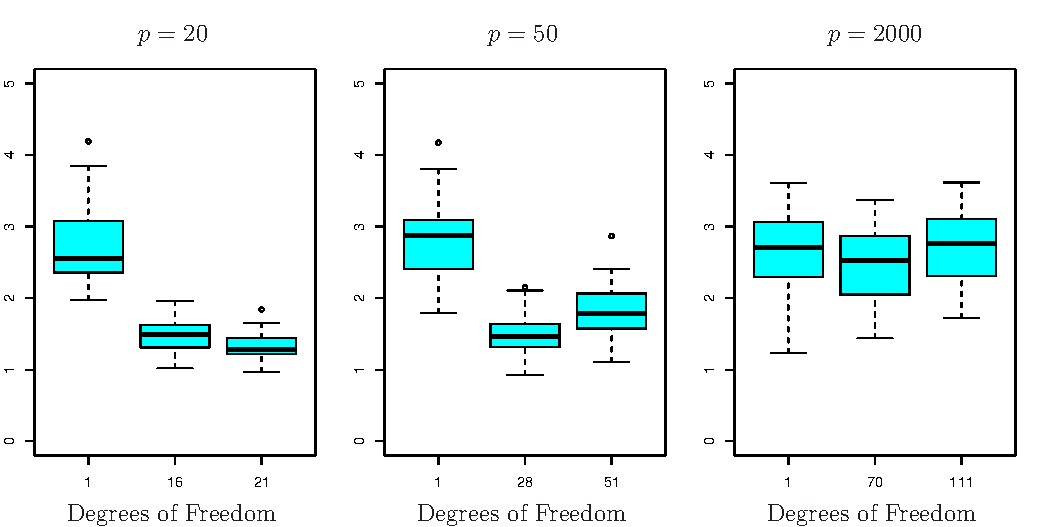
\includegraphics[width=0.92\textwidth,height=0.62\textheight,keepaspectratio]{6_24.pdf}
  \end{center}
  Lasso continues to work even when $p \gg n$, provided the truth is
  sparse (only a few non-zero $\beta_j$).
  \islpsource{Figure 6.24}
\end{frame}


% ============================================================
\section{Python Lab}

\begin{frame}{Python lab --- run it live in the notebook}
  \begin{labnote}[Companion notebook: \texttt{chapter\_06\_lab.ipynb}]
    The code in this section is meant to be \textbf{demonstrated live}. Open the companion Jupyter notebook and run it cell by cell:
    \begin{itemize}
      \item best-subset and forward stepwise selection on Hitters;
      \item ridge regression and the lasso (coefficient paths);
      \item principal-components and partial-least-squares regression.
    \end{itemize}
    Data loads via the \texttt{ISLP} package or the bundled CSV files; the notebook ends with hands-on exercises.
  \end{labnote}
\end{frame}


% ============================================================

\begin{frame}[fragile]{Best subset and stepwise (manual)}
  \begin{lstlisting}
import statsmodels.api as sm, itertools
from ISLP import load_data
Hitters = load_data("Hitters").dropna()      # drop rows with NA salary
y = Hitters["Salary"]                         # response
preds = [c for c in Hitters.columns if c not in ("Salary",)]

best = {}
for k in range(1, 6):                         # model sizes k = 1..5
    best_rss = None
    for combo in itertools.combinations(preds, k):  # all C(p,k) subsets
        X = sm.add_constant(Hitters[list(combo)])
        rss = sm.OLS(y, X).fit().ssr          # training RSS of subset
        if best_rss is None or rss < best_rss:
            best_rss, best_combo = rss, combo  # keep best model per size
    best[k] = (best_combo, best_rss)
  \end{lstlisting}
\end{frame}

\begin{frame}[fragile]{Ridge regression}
  \begin{lstlisting}
from sklearn.linear_model import RidgeCV
from sklearn.preprocessing import StandardScaler
import numpy as np

X = StandardScaler().fit_transform(Hitters[preds])  # standardise first!
y = Hitters["Salary"].values
ridge = RidgeCV(alphas=np.logspace(-2, 4, 50)).fit(X, y)  # CV over grid
print("best alpha:", ridge.alpha_)           # lambda chosen by CV
print(dict(zip(preds, ridge.coef_)))         # all coefs stay nonzero
  \end{lstlisting}
\end{frame}

\begin{frame}[fragile]{The lasso}
  \begin{lstlisting}
from sklearn.linear_model import LassoCV

lasso = LassoCV(alphas=np.logspace(-3, 1, 50), cv=10,  # 10-fold CV
                random_state=0).fit(X, y)    # fit path over alpha grid
print("best alpha:", lasso.alpha_)           # lambda chosen by CV
nonzero = [(p, c) for p, c in zip(preds, lasso.coef_) if c != 0]
print(nonzero)                               # only the survivors
  \end{lstlisting}
\end{frame}

\begin{frame}[fragile]{Principal components regression}
  \begin{lstlisting}
from sklearn.decomposition import PCA
from sklearn.linear_model  import LinearRegression
from sklearn.pipeline      import Pipeline
from sklearn.model_selection import cross_val_score

scores = []
for M in range(1, len(preds) + 1):           # try every component count
    pcr = Pipeline([("pca", PCA(n_components=M)),  # M principal comps
                    ("ols", LinearRegression())])  # then plain OLS
    s = -cross_val_score(pcr, X, y, cv=10,   # 10-fold CV MSE
                          scoring="neg_mean_squared_error").mean()
    scores.append(s)                         # CV curve over M
  \end{lstlisting}
\end{frame}

\begin{frame}[fragile]{Exercise 6.7 --- CV Ridge and Lasso on Hitters [Python]}
  \begin{exercise}
    On the \texttt{Hitters} data (predict \texttt{Salary}), (i) fit
    lasso with a cross-validated $\lambda$ on standardised predictors,
    (ii) report the selected $\lambda$, and (iii) list which features the
    lasso keeps versus drops. Contrast with ridge. What do the results
    tell you?
  \end{exercise}
\end{frame}

\begin{frame}[fragile]{Solution --- Exercise 6.7 (1/2)}
  \begin{lstlisting}
import numpy as np, pandas as pd
from sklearn.linear_model  import LassoCV, RidgeCV
from sklearn.preprocessing import StandardScaler

df = pd.read_csv("../../ALL CSV FILES - 2nd Edition/Hitters.csv").dropna()
y = df["Salary"].values
X_raw = pd.get_dummies(df.drop(columns=["Salary"]), drop_first=True)
preds = X_raw.columns
X = StandardScaler().fit_transform(X_raw)    # standardise predictors

lasso = LassoCV(cv=10, random_state=0, max_iter=10000).fit(X, y)  # CV
print("lasso alpha:", round(lasso.alpha_, 3))  # chosen lambda
kept    = [p for p, c in zip(preds, lasso.coef_) if abs(c) > 1e-8]
dropped = [p for p, c in zip(preds, lasso.coef_) if abs(c) <= 1e-8]
print("kept   :", kept)      # features the lasso retains
print("dropped:", dropped)   # features zeroed out exactly
  \end{lstlisting}
\end{frame}

\begin{frame}[fragile]{Solution --- Exercise 6.7 (2/2)}
  \begin{lstlisting}
ridge = RidgeCV(alphas=np.logspace(-2, 4, 50)).fit(X, y)  # CV grid
print("ridge alpha:", round(ridge.alpha_, 3),
      "-- nonzero coefs:", int(np.sum(np.abs(ridge.coef_) > 1e-8)))  # all p
  \end{lstlisting}
  \begin{solutionbox}[Expected result and interpretation]
    The lasso selects a moderate $\lambda$ and \emph{drives several
    coefficients to exactly zero} --- typically it keeps strong career
    and recent-performance predictors (e.g.\ \texttt{CRBI},
    \texttt{Hits}, \texttt{Walks}, \texttt{PutOuts},
    \texttt{DivisionW}) and drops weak, redundant ones. Ridge, by
    contrast, keeps \emph{all} predictors nonzero (only shrinks them).
    Takeaway: lasso yields a sparse, more interpretable model performing
    automatic variable selection, whereas ridge stabilises the fit while
    retaining every predictor. Choose based on whether sparsity or
    keeping all predictors is preferred.
  \end{solutionbox}
\end{frame}


\begin{frame}[fragile]{Extended Exercise 6.3 --- CV Ridge and Lasso Test MSE on Hitters [Python]}
  \begin{longexercise}
    On the \texttt{Hitters} data (predict \texttt{Salary}; drop missing
    salaries; dummy-encode \texttt{League}, \texttt{Division},
    \texttt{NewLeague}):
    \begin{enumerate}
      \item Split into train/test, standardise predictors \emph{using the
            training set only}, and cross-validate to choose $\lambda$ for
            both ridge and lasso.
      \item Report each chosen $\lambda$, the \emph{test} MSE, and how
            many coefficients are non-zero.
      \item List the predictors the lasso drops and contrast ridge vs.\
            lasso.
    \end{enumerate}
  \end{longexercise}
\end{frame}

\begin{frame}[fragile]{Solution --- Extended Exercise 6.3 (1/3)}
  \begin{lstlisting}
import numpy as np, pandas as pd
from sklearn.model_selection import train_test_split
from sklearn.preprocessing  import StandardScaler
from sklearn.linear_model   import RidgeCV, LassoCV
from sklearn.metrics        import mean_squared_error

D  = "../../ALL CSV FILES - 2nd Edition/"
df = pd.read_csv(D+"Hitters.csv").dropna(subset=["Salary"])  # drop NA y
y  = df["Salary"].values
X  = pd.get_dummies(df.drop(columns=["Salary"]),
                    drop_first=True).astype(float)  # encode factors
Xtr, Xte, ytr, yte = train_test_split(X.values, y,
                        test_size=0.33, random_state=1)  # 2/3-1/3 split
sc = StandardScaler().fit(Xtr)      # fit on TRAIN only: no leakage
Xtr, Xte = sc.transform(Xtr), sc.transform(Xte)  # apply to both sets
  \end{lstlisting}
\end{frame}

\begin{frame}[fragile]{Solution --- Extended Exercise 6.3 (2/3)}
  \begin{lstlisting}
ridge = RidgeCV(alphas=np.logspace(-2, 4, 50)).fit(Xtr, ytr)  # CV grid
lasso = LassoCV(cv=10, max_iter=100000,
                random_state=0).fit(Xtr, ytr)   # 10-fold CV for lambda

for name, m in [("ridge", ridge), ("lasso", lasso)]:
    mse = mean_squared_error(yte, m.predict(Xte))   # TEST-set MSE
    nz  = int(np.sum(np.abs(m.coef_) > 1e-8))       # nonzero coefs
    print(name, "lambda=", round(m.alpha_, 3),
          "testMSE=", round(mse, 0), "nonzero=", nz)

dropped = [c for c, w in zip(X.columns, lasso.coef_)
           if abs(w) <= 1e-8]                       # zeroed by lasso
print("lasso drops:", dropped)
  \end{lstlisting}
\end{frame}

\begin{frame}{Solution --- Extended Exercise 6.3 (3/3)}
  \begin{solutionbox}[Expected result and interpretation]
    With $n=263$, $p=19$ and this split you should see roughly:
    \begin{itemize}
      \item \textbf{Ridge}: $\lambda\approx0.1$, test MSE
            $\approx1.2\times10^5$, \emph{all $19$ coefficients
            non-zero}.
      \item \textbf{Lasso}: $\lambda\approx0.8$, test MSE
            $\approx1.2\times10^5$, about $16$ non-zero --- it drops
            \texttt{Years}, \texttt{CRBI}, \texttt{Errors} (weak or
            redundant given the correlated career totals).
    \end{itemize}
    \textbf{Contrast.} Both attain very similar test error, but the lasso
    reaches it with a \emph{sparser, more interpretable} model (automatic
    variable selection), whereas ridge keeps and merely shrinks all
    predictors. Exact numbers shift with the split/seed; the qualitative
    message --- lasso selects, ridge keeps all --- is stable.
  \end{solutionbox}
\end{frame}

% ============================================================
\section{Summary}
% ============================================================

\begin{frame}{Chapter 6 in one slide}
  \begin{block}{What we accomplished}
    Three families of methods that turn the linear model into a
    workhorse for high-dimensional and sparse problems.
  \end{block}
  \begin{itemize}
    \item Subset selection (best, forward, backward).
    \item Shrinkage (ridge, lasso, elastic net).
    \item Dimension reduction (PCR, PLS).
    \item Honest tuning via cross-validation throughout.
  \end{itemize}
\end{frame}

\begin{frame}{Key formulas at a glance}
  \footnotesize
  \begin{description}
    \item[$C_p$] $C_p=\dfrac1n\big(\mathrm{RSS}+2d\hat\sigma^2\big)$ \quad (lower is better).
    \item[AIC / BIC] $\mathrm{AIC}\propto \mathrm{RSS}+2d\hat\sigma^2$; \quad $\mathrm{BIC}=\dfrac1n\big(\mathrm{RSS}+\log(n)\,d\,\hat\sigma^2\big)$.
    \item[Adjusted $R^2$] $1-\dfrac{\mathrm{RSS}/(n-d-1)}{\mathrm{TSS}/(n-1)}$.
    \item[Ridge ($\ell_2$)] $\min_\beta\ \mathrm{RSS}+\lambda\sum_{j=1}^p\beta_j^2$ \quad (shrinks, keeps all predictors).
    \item[Lasso ($\ell_1$)] $\min_\beta\ \mathrm{RSS}+\lambda\sum_{j=1}^p|\beta_j|$ \quad (shrinks and selects: some $\hat\beta_j=0$).
    \item[Tuning] choose $d$ or $\lambda$ by cross-validation.
  \end{description}
\end{frame}

\begin{frame}{Vocabulary checklist}
  \footnotesize
  \begin{tabular}{ll}
    \toprule
    \textbf{Term} & \textbf{Meaning} \\
    \midrule
    Best subset & Search all $\binom{p}{k}$ models for each $k$ \\
    Forward / backward & Greedy add / drop one predictor at a time \\
    $C_p$ / AIC / BIC & Penalised RSS criteria for model size \\
    Adjusted $R^2$ & $R^2$ penalised for the number of predictors \\
    Ridge ($\ell_2$) & Penalty $\lambda \sum \beta_j^2$ \\
    Lasso ($\ell_1$) & Penalty $\lambda \sum |\beta_j|$ \\
    Elastic net & Mix of $\ell_1$ and $\ell_2$ penalties \\
    Tuning parameter $\lambda$ & Strength of the penalty \\
    PCR & Regression on principal components of $\mathbf{X}$ \\
    PLS & Regression on directions correlated with $Y$ \\
    Sparsity & Many estimated $\beta_j$ exactly zero \\
    \bottomrule
  \end{tabular}
\end{frame}

\begin{frame}{Decision rules of thumb}
  \begin{itemize}
    \item Always standardise predictors before ridge / lasso / PCR /
          PLS.
    \item Choose $\lambda$ by 10-fold CV; consider the
          one-standard-error rule for parsimony.
    \item Use BIC for parsimonious model selection; AIC / $C_p$ for
          predictive accuracy.
    \item In $p > n$ regimes: ridge or lasso is mandatory.
    \item Re-fit OLS on the lasso-selected variables (``relaxed lasso'')
          if you want unbiased coefficients with the sparse support.
  \end{itemize}
\end{frame}

\begin{frame}{Common pitfalls}
  \begin{alertblock}{Don't}
    \begin{enumerate}
      \item Apply lasso / ridge without standardising.
      \item Treat post-selection $p$-values as valid (Ch.~13).
      \item Use AIC / BIC for high-dimensional data --- they assume
            $n \gg p$.
      \item Tune $\lambda$ on the same data you evaluate on.
      \item Throw away PCs based purely on variance --- a low-variance
            PC can be highly predictive of $Y$.
      \item Forget that PCR ignores $Y$; PLS is the supervised
            alternative.
    \end{enumerate}
  \end{alertblock}
\end{frame}

\begin{frame}{Connections to the rest of the course}
  \begin{itemize}
    \item Ch.~3: linear regression with no penalty.
    \item Ch.~5: how to choose $\lambda$ honestly via CV.
    \item Ch.~7: GAMs are an additive ridge-like extension.
    \item Ch.~8: random forests / boosting handle high-dim differently.
    \item Ch.~10: deep nets use weight decay (ridge in disguise).
    \item Ch.~13: post-selection inference and the lasso.
  \end{itemize}
\end{frame}

\begin{frame}{Self-check questions}
  \begin{enumerate}
    \item Why does ridge regression always have a unique solution?
    \item Why can lasso set coefficients to exactly zero, but ridge
          cannot? Sketch the unit balls.
    \item For two perfectly correlated predictors, what does ridge do?
          What does lasso do? What does elastic net do?
    \item Compute the ridge estimate when $\mathbf{X}^\top\mathbf{X} = I$
          --- a clean special case.
    \item PCR ignores $Y$ when forming components. When can this hurt
          and when does it help?
    \item Outline the one-standard-error rule.
  \end{enumerate}
\end{frame}

\begin{frame}{Eight things to remember}
  \begin{enumerate}
    \item Subset selection: clean conceptually but combinatorial.
    \item Stepwise selection: greedy and fast.
    \item Ridge: $\ell_2$ penalty $\to$ smooth shrinkage, no zeros.
    \item Lasso: $\ell_1$ penalty $\to$ sparse solutions.
    \item Always standardise before shrinkage.
    \item Choose $\lambda$ by cross-validation.
    \item PCR / PLS: dimension reduction; PLS uses $Y$.
    \item In high dimensions, regularisation is essential.
  \end{enumerate}
\end{frame}

\begin{frame}{What's next}
  Chapter 7: \emph{Moving Beyond Linearity}.
  \begin{itemize}
    \item Polynomial and step functions.
    \item Regression splines and smoothing splines.
    \item Local regression.
    \item Generalised additive models.
  \end{itemize}
\end{frame}

\end{document}
